\section{Object Recognition}
As mentioned in the analysis, object recognition algorithms can be tedious to do by hand.
Although the initial target of the device may be a simple and easily recognizable object, the intent is to create a system that can potentially find and track more complicated targets.
Therefore more sophisticated object recognition methods will be utilized from the very beginning.

\subsection{OpenCV}
One option is to simply utilize the highly popular OpenCV library.
OpenCV is an open source computer vision library, that comes with ready to use object tracking functionality.
% Write more

\subsubsection{GOTURN}


\subsection{Neural Networks}

A neural network is as the name implies a network of neurons.
It is known from the brain, in which a neural network is used to make decisions.
However, in computer science neural network refers to an artificial neural network.
An artificial neural network is an artificial version of a neural network, which is inspired by the neural network present within the brain.
The basic idea within a neural network, is that a neuron will receive some input, do some calculations, and then transmit the result to connected neurons.

Neural networks is one of the most popular technologies used within machine learning.
It is however also one of the more complicated methods, so it should be considered whether some of the simpler approaches could be utilized, before deciding on the neural network.
One of the reasons neural networks are especially interesting in this case, is its ability to recognize patterns.
Pattern recognition is a fundamental part of object recognition making neural networks an obvious option.


\subsubsection{Convolutional Neural Network}
Convolutional neural networks (CNN) are often used for image classification, and is the most popular type of neural network in regards to object detection.
In challenges such as LSVCR\footnote{Imagenet Large Scale Visual Recognition Challenge} the majority of the entries are done using CNN %[http://www.image-net.org/challenges/LSVRC/2014/results]. 
A CNN is a neural network in which neurons are grouped into layers.
An input layer, an output layer and a number of so called hidden layers.
The goal of the hidden layers are to transform the input data into the expected output data.
It does this by doing abstractions within each layer, breaking a complex problem up into smaller and more trivial subproblems.

In terms of object recognition, an example could be face recognition.
The first layer could recognize lines, edges or similar low level features.
The following layers could then detect increasingly complicated patterns, ending at some layer, in which one neuron would transmit a signal if a nose is present in the image, and another neuron to transmit if a mouth is present.



\begin{figure}[H]
	\centering
	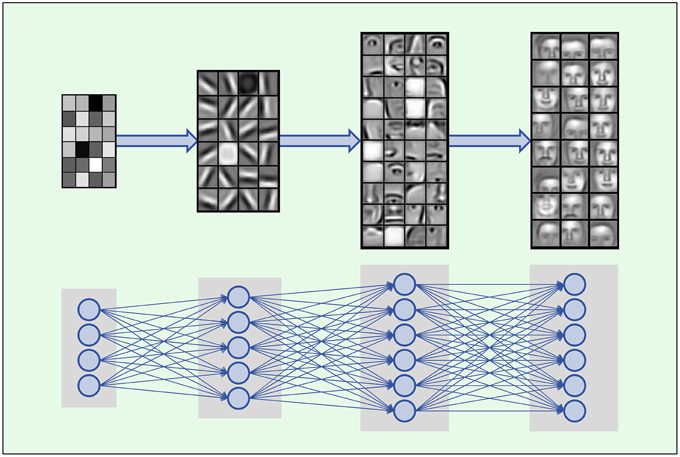
\includegraphics[scale=0.40]{images/cnn_face.jpg}
	\caption{
		A simplified example of the abstractions within a CNN.
	}
	\label{fig:face_cnn}
\end{figure}
 
However, it is important to understand, that this is not necessarily the patterns that a CNN will detect within its layers.
Actually it is far more likely, that the layers will recognize something that to a human has no relation to a face.
But the computer will have found a correlation between these seemingly random patterns, and a face.

Often used along with pooling.

CNNs are very good at classification. 
This means it can answer yes or no to whether the image is of a car.
Now the question is whether it can be used to figure out the position of the objects within the image.
  

% Seems to be very good for still images, but not so much for video tracking https://en.wikipedia.org/wiki/Convolutional_neural_network#Video_analysis

\subsubsection{Regional Convolutional Neural Network}

\subsection{You Only Look Once}
You Only Look Once (YOLO) ...

\subsection{Tensorflow}


% Things to check / consider writing about
% https://en.wikipedia.org/wiki/Computer_vision#Recognition
% https://en.wikipedia.org/wiki/Video_tracking
% Kernel-based tracking
% Contour tracking
% https://en.wikipedia.org/wiki/Kalman_filter
% Particle filter
% https://en.wikipedia.org/wiki/Outline_of_object_recognition
% real-time: triangulate each frame and measure the persistence of selected triangles relative to their location in each successive frame. Microprocessors such as the raspberry pi are fast enough so that triangulation and triangle measurement can be done in a few milliseconds.
% ^^ Few miliseconds (Sounds like maybe around 5ms, would alow for updating robot position 20 times a second (capture 20 fps from the camera too). Which could be a goal to aim at (RTS: scheduling bla bla, update canon position 20 times pr second...))
% Would be cool in RTS part to integrate some functionality to handle if camera data is not ready within the 5 ms, or if the device is not ready to handle input after 5 ms. The MI part could be coded to update each 5 ms.